\documentclass[slidestop,compress,red]{beamer}
\usepackage{graphicx}

\usetheme{Antibes}

\usepackage{fontspec}
\usepackage{xltxtra}
\setsansfont{Ubuntu}

\beamertemplatenavigationsymbolsempty

\definecolor{light-gray}{gray}{0.7}

\title{Escalator}
\subtitle{Flexible On-Call Benachrichtigung}
\author{Hermann Loose}
\date{10.02.2012}

\begin{document}

\frame[plain]{\titlepage}

\begin{frame}[plain]
  \frametitle{Motivation}
  \begin{flushleft}
    \emph{„do one thing and do it well“}
  \end{flushleft}
  \begin{itemize}
    \item automatische Eskalation von Ereignissen
    \begin{itemize}
      \item an rotierende Bereitschaftsdienste
      \item über flexible Wege der Benachrichtigung
    \end{itemize}
  \end{itemize}
  \begin{flushleft}
    \emph{„write programs that work together“}
  \end{flushleft}
  \begin{itemize}
    \item REST-Schnittstelle für Ereignisse
    \begin{itemize}
      \item Monitoring, Ticket-System, …
    \end{itemize}
    \item unkomplizierte, erweiterbare Backends
    \begin{itemize}
      \item prototypisch: Email, Android
      \item denkbar: Boxcar (iOS), SMS, XMPP, …
    \end{itemize}
  \end{itemize}
\end{frame}

\begin{frame}[c,plain]
  \frametitle{Fokus}
  \begin{itemize}
    \item schlank
    \item generisch
    \begin{itemize}
      \item nicht: Ersatz für Nagios, etc.
    \end{itemize}
    \item self-service
    \begin{itemize}
      \item Wege und zeitl. Abstände der Benachrichtigung
      \item perspektivisch: z.B. Rotationen mit Diensttausch
    \end{itemize}
  \end{itemize}
\end{frame}

\begin{frame}[c,plain]
  \frametitle{Konzept}
  \begin{itemize}
    \item Ereignisse landen in einer Eskalationsstrategie
    \item Eskalationsstrategien haben eine Hierarchie von Rotationen
    \item bis ein Ereignis akzeptiert wird, steigt es in der Hierarchie in Zeitschritten auf
    \item Rotationen umfassen Nutzer, von denen jeweils einer Bereitschaftsdienst hat
    \item Nutzer definieren pro Rotation, wie sie (schrittweise) benachrichtigt werden wollen
  \end{itemize}
\end{frame}

\begin{frame}[c,plain]
  \frametitle{bisherige Arbeit}
  \begin{itemize}
    \item Backend / Web-Frontend (Rails 3.1.3)
    \begin{itemize}
      \item Jobs für Eskalation und Rotation
      \item Email- und Android-Backend
      \item Authentifizierung \& Authorisierung
    \end{itemize}
    \item Android (2.2)
    \begin{itemize}
      \item grundlegender C2DM Workflow
      \item prototypische Benachrichtigungen
    \end{itemize}
  \end{itemize}
\end{frame}

\begin{frame}[c,plain]
  \frametitle{Zukunft}
  \begin{columns}
    \begin{column}{0.4\textwidth}
      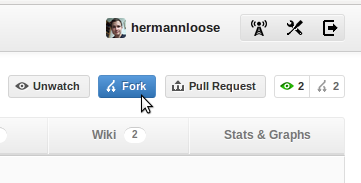
\includegraphics[width=12em]{fork}
    \end{column}
    \begin{column}{0.4\textwidth}
      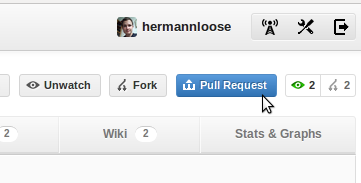
\includegraphics[width=12em]{pullrequest}
    \end{column}
  \end{columns}
  \begin{itemize}
    \item \texttt{https://github.com/hermannloose/escalator}
    \item \texttt{https://github.com/hermannloose/escalator-android}
  \end{itemize}
\end{frame}

\end{document}
